\section{Introduction}

The \textit{proceedings} are the records of a conference.\footnote{This
  is a footnote}  ACM seeks
to give these conference by-products a uniform, high-quality
appearance.  To do this, ACM has some rigid requirements for the
format of the proceedings documents: there is a specified format
(balanced double columns), a specified set of fonts (Arial or
Helvetica and Times Roman) in certain specified sizes, a specified
live area, centered on the page, specified size of margins, specified
column width and gutter size.

\section{Related Work}

\section{Experiment Setup}
%123456789123456789123456789123456789123456789123456789123456789
In this Section, we describe the experimental approach we 
used in order to perform our research and retrieve our 
measurements. 
Initially, we provide information about our dataset 
and the ways we decided to select our tasks and 
refine it.
Furthermore, we explain the setup up of our experimental 
platform, the additional hardware tools, and the software 
tools used to conduct this research. 
Moreover, we argue on the selected tasks and programming 
languages we used and the way re refined our dataset.

\subsection{Dataset}
%123456789123456789123456789123456789123456789123456789123456789
In the context of study, we used Rosetta 
Code,\footnote{http://rosettacode.org/wiki/Rosetta\_Code} a 
publicly available programming chromatography site that offers 
851 tasks, 230 draft tasks, and a collection of 658 different 
programming languages. In general, not all of (and cannot) tasks 
are implemented in all languages. 
We found and downloaded a git hub repository\footnote{https://github.com/acmeism/RosettaCodeData} 
which contains all the currently implemented tasks found on 
Rosetta Code website.

%123456789123456789123456789123456789123456789123456789123456789
For selecting the highly used programming languages, we made use 
of tiobe,\footnote{https://www.tiobe.com/tiobe-index/} a software 
quality company.
By making use of a formula\footnote{https://www.tiobe.com/tiobe-index/programming-languages-definition/}, 
25 of the highest ranked search engines (according to Alexa),\footnote{http://www.alexa.com/} 
and a number of requirements enlisted for programming languages, 
tiobe provides a search query for index rating of the most popular 
programming languages around the web for each month. 
Initially, we decided of choosing the top 15 programming languages 
as enlisted for June 2017. 
From the current list, we excluded programming languages such as 
Delphi and Assembly. 
In contrast, we included Rust in our dataset which a memory safe 
programming language and is gaining popularity in the web. \
Therefore, we ended up with 14 programming languages as illustrated 
in Table~\ref{Languages_Compilers_and_Interpreters}.

%123456789123456789123456789123456789123456789123456789123456789 
In terms of selecting tasks, we developed a shell script (more 
details in Subsection~\ref{software_components}) to identify 
which of the 851 tasks offers the most implementations for the 
programming languages of our selection. 
To refine further our dataset we used the following steps: 

\begin{enumerate}
	\item [$\bullet$] We excluded implemented tasks that are using 
	external libraries. 
	Since we would like to exploit the energy dissipation of 
	simple every day tasks, we decided to exclude form our dataset 
	the use of tasks requiring external libraries. 
	\item [$\bullet$] Some of the tasks offers more that one implementation 
	for the same programming languages. 
	Thus, we had to drive manually through each directory and remove 
	them until we have only one that is consistent with the other 
	implementation. 
	For example, palindrome in recursion we removed the iterative 
	implementations. 
	\item [$\bullet$] The Java file's names were 
	different from the public class names which results to compilation 
	error if not change accordingly. 
	\item [$\bullet$] Some of the implementations didn't have main 
	classes, nor the same data with other tasks. 
	Therefore, we change the source code to offer consistency.
	\item [$\bullet$] Some of the tasks are relatively small and may 
	finish faster than 1 second which makes it impossible for our 
	power analyzer to capture those results. 
	Therefore, we added all the selected tasks in a loop to iterate them 
	a million of times. 
\end{enumerate}


\subsection{Hardware and Software components}

\subsubsection{Hardware Components}
%123456789123456789123456789123456789123456789123456789123456789 
The physical tools composed mainly from a portable personal 
computer and a real-time electricity usage monitoring tool.
Our system's specifications are depicted in Table~\ref{laptop_specs}. 
The real-time power usage tools we used is the Watts Up Pro ({\sc wup}).\footnote{https://www.wattsupmeters.com/secure/products.php?pn=0} 

In general, there are two venues for retrieving energy consumption 
from a computer-system: on one hand, by indirect energy measurements 
through estimation models or performance counters, core component 
of software monitoring tools, on the other hand, via direct measurement, 
hardware power analyzers and sensors.  
However, each approach has it own pitfalls such as: coarse-grained 
measurements for the whole systems energy consumption and low sampling 
rate for direct measurements case and inaccuracy, lack of interoperability, 
and additional system overhead while indirect measurements. 
Therefore, in our research we decided to retrieve our energy consumption 
measurements using direct approach such as {\sc wup} since our 
tasks are relatively short in terms of source-code lines.


In regards to {\sc wup}, it offers accuracy of \textpm1.5\% and 
as maximum sampling rate of 1 second. 
In order to retrieve power-related measurements from the {\sc wup} 
we used a software available in a Git repository.\footnote{https://github.com/pyrovski/watts-up}
This software helped us retrieve measurements such as timestamps, 
watts, volts, amps, etc. through a mini {\sc usb} interface after 
we integrated its code in our script that runs all the tasks.

\subsubsection{Software Components} \label{software_components}
%123456789123456789123456789123456789123456789123456789123456789 
To extract data, manage, and use our Rosetta Code Repository, 
we developed a number of shell scripts as enlisted below and are 
publicly available on our Git repository.\footnote{https://github.com/stefanos1316/Rosetta-Code-Research} 

\begin{enumerate}
	\item [$\bullet$] \textbf{script.cleanAll}, removes the current instance 
	of Tasks in the current working directory and copy the new one found 
	from in the parent directory. 
	\item [$\bullet$] \textbf{script.fromUpperToLower}, changes the current 
	instance of Tasks directory tree's letters from upper to lower 
	case to offer consistency for our scripts. 
	\item [$\bullet$] \textbf{script.findCommonTasksInLanguages}, provides 
	a list of tasks with the amount of programming language implementations.
	\item [$\bullet$] \textbf{script.createNewDataSet}, filters the Rosetta 
	Code current dataset and removes programming languages and tasks not 
	added as command line arguments.
	\item [$\bullet$] \textbf{script.compileTasks}, compiles all tasks found 
	under the Tasks' directory and produces error reports in a task fails to 
	compile.
	\item [$\bullet$] \textbf{script.executeTasks}, executes all the tasks' 
	implementations found in under Tasks directory.
	\item [$\bullet$] \textbf{script.plotGraphs}, after retrieving our data 
	we use this script to plot our graphs.
\end{enumerate}

%123456789123456789123456789123456789123456789123456789123456789 
Note that most of the scripts offer the \textit{--help} option 
that shows a list of available command line arguments in order 
use our scripts.
Moreover, users are suggested not to change the folders name or 
locations since most of our scripts are making use of them. 

For plotting our graphs we used FeedGnuplot,\footnote{http://search.cpan.org/~dkogan/feedgnuplot-1.44/bin/feedgnuplot} 
an open-source general purpose pipe-oriented plotting tool. 
To use our script for plotting graphs, someone has to provide a 
columned file with energy related measurements.

\begin{table}
		\begin{threeparttable}
	\caption{System hardware and software specifications}
	\label{laptop_specs}
	\begin{tabular}{cl}
		\toprule
		&Description\\
		\midrule
		Hardware	& HP EliteBook 840 G3, Intel Core i7-6500U \\
					& (2 physical cores of 2.5 GHz), 8 GB DDR4  \\
					& memory, 256 GB {\sc ssd}  hard disk \\
		Operating  System & Fedora 25 kernel version 4.11.5-200  \\			
		Software 	& {\sc wup} software (retrieving measurements \\
					& from the device), bash script, Java, R, \\
					& feedGnuplot \\
		\bottomrule
	\end{tabular}
	\end{threeparttable}
\end{table}

\begin{table}
	\begin{threeparttable}
	\caption{Programming Languages, Compilers and Interpreters}
	\label{Languages_Compilers_and_Interpreters}
	\begin{tabular}{cl}
		\toprule
		Programming Languages & Compilers \ Interpreters \\
		\midrule
		C, C++	& gcc version 6.3.1 20161221- \\
				& (Red Hat 6.3.1-1) (GCC) \\
		C\#		& mono version 4.4.2.0 (mics)\tnote{a} \\
		Go		& go version go1.7.5 linux/amd64 \\
		Java	& javac version 1.8.0\_131 \\
		JavaScript & node version 6.10.3 \\
		Perl	& perl version 5.24.1 \\
		Php		& php version 7.0.19 \\
		Python	& python version 2.7.13 \\
		R		& Rscript version 3.3.3 \\
		Ruby	& ruby version 2.3.3p222 \\
		Rust	& rustc version 1.18.0 \\
		Swift 	& swift version 3.0.2\tnote{b} \\
		{\sc vb.net} & vbnc version 0.0.0.5943\tnote{c} \\
		\bottomrule
	\end{tabular}
	\begin{tablenotes}
		\begin{small}
			\item[a] {https://www.codetuts.tech/compile-c-sharp-command-line/}
			\item[b] {https://github.com/FedoraSwift/fedora-swift2/releases/tag/v0.0.2}
			\item[c] {http://www.mono-project.com/docs/about-mono/languages/visualbasic/}
		\end{small}
	\end{tablenotes}
	\end{threeparttable}
\end{table}


\subsection{Retrieving Energy Measurements} 
%123456789123456789123456789123456789123456789123456789123456789 
As an initial step for our experiment, we shut down background 
process, as suggested by Hindle[...], found in modern {\sc os}s such as disk 
defragmentation, virus scanning, {\sc cron} jobs, automatic updates, 
disk indexing, document indexing, {\sc rss} feed updates, etc. to 
shorten some noise in our measurements. 
In addition, we set the network connection to flight mode and 
also reduced the brightness of the screen.
By making the following steps we reduced our platform's idle 
power usage from 8,6 watts to 5.8 watts. 
We estimated that after an {\sc os} (Operating System) is launched 
it's necessary to wait for a short time to reach a 
\textit{stable condition}.

%123456789123456789123456789123456789123456789123456789123456789 
After reaching \textit{stable condition}, we launched our main 
script \textit{i.e.,} \textbf{script.executeTasks}, that executes 
all the tasks implemented in different programming languages. 
While doing so, it retrieves power consumption and run-time 
performance measurements from {\sc wup} and through command 
time\footnote{https://linux.die.net/man/1/time} and stores them 
in timestamped directories which we are using later to plot 
our results. 
Between each executing of a task, we added a 
sleep\footnote{http://man7.org/linux/man-pages/man3/sleep.3.html} 
period of three minutes. 
The time gap purpose is to ensure our experimental platform 
reached a stable condition,\textit{e.g.,} the {\sc cpu} is cooled 
down and the fan is no longer consuming more power, to avoid 
unnecessary noise in our measurements.

\section{Results and Discussion}
Graphs for programming languages using compilers and interpreters

\section{Threats of validity}

\section{Conclusion and Future Work}
Two Venues, Academic and Industrial.
She under the curtain and shed light... 
Compare PL in different CPU architectures such as 
ARM and AMD.
More tasks and different configuration and optimizaiton 
flags.
Collect resource usage and system calls to identify 
relationship among them.

Future plans, micro-services proposition of tasks or 
programming languages after identifying the reasons

\subsection{Math Equations}
You may want to display math equations in three distinct styles:
inline, numbered or non-numbered display.  Each of
the three are discussed in the next sections.

\subsubsection{Inline (In-text) Equations}
A formula that appears in the running text is called an
inline or in-text formula.  It is produced by the
\textbf{math} environment, which can be
invoked with the usual \texttt{{\char'134}begin\,\ldots{\char'134}end}
construction or with the short form \texttt{\$\,\ldots\$}. You
can use any of the symbols and structures,
from $\alpha$ to $\omega$, available in
\LaTeX~\cite{Lamport:LaTeX}; this section will simply show a
few examples of in-text equations in context. Notice how
this equation:
\begin{math}
  \lim_{n\rightarrow \infty}x=0
\end{math},
set here in in-line math style, looks slightly different when
set in display style.  (See next section).

\subsubsection{Display Equations}
A numbered display equation---one set off by vertical space from the
text and centered horizontally---is produced by the \textbf{equation}
environment. An unnumbered display equation is produced by the
\textbf{displaymath} environment.

Again, in either environment, you can use any of the symbols
and structures available in \LaTeX\@; this section will just
give a couple of examples of display equations in context.
First, consider the equation, shown as an inline equation above:
\begin{equation}
  \lim_{n\rightarrow \infty}x=0
\end{equation}
Notice how it is formatted somewhat differently in
the \textbf{displaymath}
environment.  Now, we'll enter an unnumbered equation:
\begin{displaymath}
  \sum_{i=0}^{\infty} x + 1
\end{displaymath}
and follow it with another numbered equation:
\begin{equation}
  \sum_{i=0}^{\infty}x_i=\int_{0}^{\pi+2} f
\end{equation}
just to demonstrate \LaTeX's able handling of numbering.

\subsection{Citations}
Citations to articles~\cite{bowman:reasoning,
clark:pct, braams:babel, herlihy:methodology},
conference proceedings~\cite{clark:pct} or maybe
books \cite{Lamport:LaTeX, salas:calculus} listed
in the Bibliography section of your
article will occur throughout the text of your article.
You should use BibTeX to automatically produce this bibliography;
you simply need to insert one of several citation commands with
a key of the item cited in the proper location in
the \texttt{.tex} file~\cite{Lamport:LaTeX}.
The key is a short reference you invent to uniquely
identify each work; in this sample document, the key is
the first author's surname and a
word from the title.  This identifying key is included
with each item in the \texttt{.bib} file for your article.

The details of the construction of the \texttt{.bib} file
are beyond the scope of this sample document, but more
information can be found in the \textit{Author's Guide},
and exhaustive details in the \textit{\LaTeX\ User's
Guide} by Lamport~\shortcite{Lamport:LaTeX}.

This article shows only the plainest form
of the citation command, using \texttt{{\char'134}cite}.

Some examples.  A paginated journal article \cite{Abril07}, an enumerated
journal article \cite{Cohen07}, a reference to an entire issue \cite{JCohen96},
a monograph (whole book) \cite{Kosiur01}, a monograph/whole book in a series (see 2a in spec. document)
\cite{Harel79}, a divisible-book such as an anthology or compilation \cite{Editor00}
followed by the same example, however we only output the series if the volume number is given
\cite{Editor00a} (so Editor00a's series should NOT be present since it has no vol. no.),
a chapter in a divisible book \cite{Spector90}, a chapter in a divisible book
in a series \cite{Douglass98}, a multi-volume work as book \cite{Knuth97},
an article in a proceedings (of a conference, symposium, workshop for example)
(paginated proceedings article) \cite{Andler79}, a proceedings article
with all possible elements \cite{Smith10}, an example of an enumerated
proceedings article \cite{VanGundy07},
an informally published work \cite{Harel78}, a doctoral dissertation \cite{Clarkson85},
a master's thesis: \cite{anisi03}, an online document / world wide web
resource \cite{Thornburg01, Ablamowicz07, Poker06}, a video game (Case 1) \cite{Obama08} and (Case 2) \cite{Novak03}
and \cite{Lee05} and (Case 3) a patent \cite{JoeScientist001},
work accepted for publication \cite{rous08}, 'YYYYb'-test for prolific author
\cite{SaeediMEJ10} and \cite{SaeediJETC10}. Other cites might contain
'duplicate' DOI and URLs (some SIAM articles) \cite{Kirschmer:2010:AEI:1958016.1958018}.
Boris / Barbara Beeton: multi-volume works as books
\cite{MR781536} and \cite{MR781537}.

A couple of citations with DOIs: \cite{2004:ITE:1009386.1010128,
  Kirschmer:2010:AEI:1958016.1958018}. 

Online citations: \cite{TUGInstmem, Thornburg01, CTANacmart}.  


\subsection{Tables}
Because tables cannot be split across pages, the best
placement for them is typically the top of the page
nearest their initial cite.  To
ensure this proper ``floating'' placement of tables, use the
environment \textbf{table} to enclose the table's contents and
the table caption.  The contents of the table itself must go
in the \textbf{tabular} environment, to
be aligned properly in rows and columns, with the desired
horizontal and vertical rules.  Again, detailed instructions
on \textbf{tabular} material
are found in the \textit{\LaTeX\ User's Guide}.

Immediately following this sentence is the point at which
Table~\ref{tab:freq} is included in the input file; compare the
placement of the table here with the table in the printed
output of this document.

\begin{table}
  \caption{Frequency of Special Characters}
  \label{tab:freq}
  \begin{tabular}{ccl}
    \toprule
    Non-English or Math&Frequency&Comments\\
    \midrule
    \O & 1 in 1,000& For Swedish names\\
    $\pi$ & 1 in 5& Common in math\\
    \$ & 4 in 5 & Used in business\\
    $\Psi^2_1$ & 1 in 40,000& Unexplained usage\\
  \bottomrule
\end{tabular}
\end{table}

To set a wider table, which takes up the whole width of the page's
live area, use the environment \textbf{table*} to enclose the table's
contents and the table caption.  As with a single-column table, this
wide table will ``float'' to a location deemed more desirable.
Immediately following this sentence is the point at which
Table~\ref{tab:commands} is included in the input file; again, it is
instructive to compare the placement of the table here with the table
in the printed output of this document.


\begin{table*}
  \caption{Some Typical Commands}
  \label{tab:commands}
  \begin{tabular}{ccl}
    \toprule
    Command &A Number & Comments\\
    \midrule
    \texttt{{\char'134}author} & 100& Author \\
    \texttt{{\char'134}table}& 300 & For tables\\
    \texttt{{\char'134}table*}& 400& For wider tables\\
    \bottomrule
  \end{tabular}
\end{table*}
% end the environment with {table*}, NOTE not {table}!

It is strongly recommended to use the package booktabs~\cite{Fear05}
and follow its main principles of typography with respect to tables:
\begin{enumerate}
\item Never, ever use vertical rules.
\item Never use double rules.
\end{enumerate}
It is also a good idea not to overuse horizontal rules.


\subsection{Figures}

Like tables, figures cannot be split across pages; the best placement
for them is typically the top or the bottom of the page nearest their
initial cite.  To ensure this proper ``floating'' placement of
figures, use the environment \textbf{figure} to enclose the figure and
its caption.

This sample document contains examples of \texttt{.eps} files to be
displayable with \LaTeX.  If you work with pdf\LaTeX, use files in the
\texttt{.pdf} format.  Note that most modern \TeX\ systems will convert
\texttt{.eps} to \texttt{.pdf} for you on the fly.  More details on
each of these are found in the \textit{Author's Guide}.

\begin{figure}
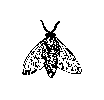
\includegraphics{fly}
\caption{A sample black and white graphic.}
\end{figure}

\begin{figure}
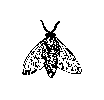
\includegraphics[height=1in, width=1in]{fly}
\caption{A sample black and white graphic
that has been resized with the \texttt{includegraphics} command.}
\end{figure}


As was the case with tables, you may want a figure that spans two
columns.  To do this, and still to ensure proper ``floating''
placement of tables, use the environment \textbf{figure*} to enclose
the figure and its caption.  And don't forget to end the environment
with \textbf{figure*}, not \textbf{figure}!

\begin{figure*}
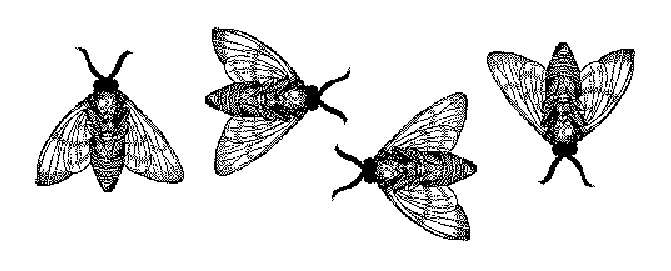
\includegraphics{flies}
\caption{A sample black and white graphic
that needs to span two columns of text.}
\end{figure*}


\begin{figure}

\includegraphics[height=1in, width=1in]{rosette}
\caption{A sample black and white graphic that has
been resized with the \texttt{includegraphics} command.}
\end{figure}

\subsection{Theorem-like Constructs}

Other common constructs that may occur in your article are the forms
for logical constructs like theorems, axioms, corollaries and proofs.
ACM uses two types of these constructs:  theorem-like and
definition-like.

Here is a theorem:
\begin{theorem}
  Let $f$ be continuous on $[a,b]$.  If $G$ is
  an antiderivative for $f$ on $[a,b]$, then
  \begin{displaymath}
    \int^b_af(t)\,dt = G(b) - G(a).
  \end{displaymath}
\end{theorem}

Here is a definition:


The pre-defined theorem-like constructs are \textbf{theorem},
\textbf{conjecture}, \textbf{proposition}, \textbf{lemma} and
\textbf{corollary}.  The pre-defined de\-fi\-ni\-ti\-on-like constructs are
\textbf{example} and \textbf{definition}.  You can add your own
constructs using the \textsl{amsthm} interface~\cite{Amsthm15}.  The
styles used in the \verb|\theoremstyle| command are \textbf{acmplain}
and \textbf{acmdefinition}.

Another construct is \textbf{proof}, for example,

\begin{proof}
  Suppose on the contrary there exists a real number $L$ such that
  \begin{displaymath}
    \lim_{x\rightarrow\infty} \frac{f(x)}{g(x)} = L.
  \end{displaymath}
  Then
  \begin{displaymath}
    l=\lim_{x\rightarrow c} f(x)
    = \lim_{x\rightarrow c}
    \left[ g{x} \cdot \frac{f(x)}{g(x)} \right ]
    = \lim_{x\rightarrow c} g(x) \cdot \lim_{x\rightarrow c}
    \frac{f(x)}{g(x)} = 0\cdot L = 0,
  \end{displaymath}
  which contradicts our assumption that $l\neq 0$.
\end{proof}

\section{Conclusions}
This paragraph will end the body of this sample document.
Remember that you might still have Acknowledgments or
Appendices; brief samples of these
follow.  There is still the Bibliography to deal with; and
we will make a disclaimer about that here: with the exception
of the reference to the \LaTeX\ book, the citations in
this paper are to articles which have nothing to
do with the present subject and are used as
examples only.
%\end{document}  % This is where a 'short' article might terminate



\appendix
%Appendix A
\section{Headings in Appendices}
The rules about hierarchical headings discussed above for
the body of the article are different in the appendices.
In the \textbf{appendix} environment, the command
\textbf{section} is used to
indicate the start of each Appendix, with alphabetic order
designation (i.e., the first is A, the second B, etc.) and
a title (if you include one).  So, if you need
hierarchical structure
\textit{within} an Appendix, start with \textbf{subsection} as the
highest level. Here is an outline of the body of this
document in Appendix-appropriate form:
\subsection{Introduction}
\subsection{The Body of the Paper}
\subsubsection{Type Changes and  Special Characters}
\subsubsection{Math Equations}
\paragraph{Inline (In-text) Equations}
\paragraph{Display Equations}
\subsubsection{Citations}
\subsubsection{Tables}
\subsubsection{Figures}
\subsubsection{Theorem-like Constructs}
\subsubsection*{A Caveat for the \TeX\ Expert}
\subsection{Conclusions}
\subsection{References}
Generated by bibtex from your \texttt{.bib} file.  Run latex,
then bibtex, then latex twice (to resolve references)
to create the \texttt{.bbl} file.  Insert that \texttt{.bbl}
file into the \texttt{.tex} source file and comment out
the command \texttt{{\char'134}thebibliography}.
% This next section command marks the start of
% Appendix B, and does not continue the present hierarchy
\section{More Help for the Hardy}

Of course, reading the source code is always useful.  The file
\path{acmart.pdf} contains both the user guide and the commented
code.

\begin{acks}
  The authors would like to thank Dr. Yuhua Li for providing the
  matlab code of  the \textit{BEPS} method. 

  The authors would also like to thank the anonymous referees for
  their valuable comments and helpful suggestions. The work is
  supported by the \grantsponsor{GS501100001809}{National Natural
    Science Foundation of
    China}{http://dx.doi.org/10.13039/501100001809} under Grant
  No.:~\grantnum{GS501100001809}{61273304}
  and~\grantnum[http://www.nnsf.cn/youngscientsts]{GS501100001809}{Young
    Scientsts' Support Program}.

\end{acks}
